ONOS\footnote{Open Network Operating System} est un contrôleur SDN open source récent (début\footnote{\url{https://en.wikipedia.org/wiki/ONOS}} en décembre 2014, la fondation Linux arrive en octobre 2015 dans le projet), écrit en Java, déployable avec Maven et utilisant Apache-Karaf comme conteneur OSGi (qui fournit entre autre l’interface utilisateur permettant l’interaction avec le contrôleur).
La version actuelle stable est Hummingbird (octobre 2016) (1.6), la prochaine annoncée est Ibis (cycles de développement d'environ 6 mois). C'est un projet essentiellement basé sur la technique \footnote{\url{http://onosproject.org/governance/}} (l'inclusion de modules est uniquement basée sur la maturité et la pertinence technique et non sur la volonté d'un acteur isolé).

Le contrôleur est structuré de la manière suivante :
\begin{figure}[h]
  	\centering
  	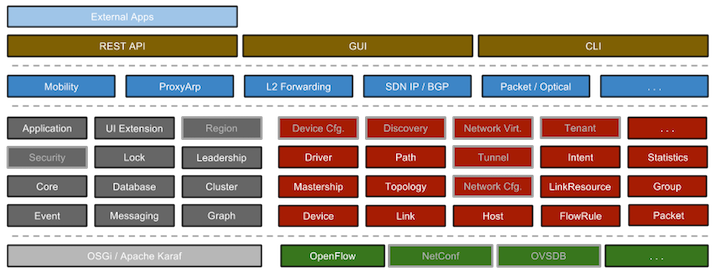
\includegraphics[width=1\textwidth]{ONOS_archi.png}
  	\caption{Architecture logicielle d'ONOS (schéma extrait du site officiel \footnotemark)}
\end{figure}

\footnotetext{\url{https://wiki.onosproject.org/display/ONOS/System+Components}}

\begin{itemize}

\item Au Sud (en gris) : Apache-Karaf qui est le conteneur OSGi et qui fournit tous les services systèmes de base.

\item Au Sud (en vert) : une API (southbound) gérant plusieurs protocoles (dont OpenFlow (toutes les versions jusqu’à la version 1.5, la version 1.6 étant en cours de prise en charge)). C’est la partie d’ONOS qui se charge de la communication avec les switchs. Il est ainsi possible de prendre en charge de nouveaux protocoles ou de nouveaux drivers.

\item Au milieu (en rouge) : tous les éléments logiciels qui fournissent au contrôleur une représentation interne du réseau physique (switchs présents, tables de flux actuelles, compteurs de paquets, liens entre équipements, ...).

\item Sur les côtés (non présent sur ce schéma) : un protocole d’échange entre contrôleurs aussi appelé interface est/ouest. Cela permet un contrôle partagé du réseau. Pour cela, des informations sur la topologie de celui-ci doivent être échangées entre contrôleurs. Le protocole en question n'est pas standardisé.

\item Au Nord (en bleu) : une API (northbound) permettant d’écrire des applications utilisant les ressources offertes par le contrôleur. Si le secure mode est activé (nous reviendrons plus en détail sur cela ultérieurement), l’ensemble des méthodes utilisables est restreint. 

\item Au Nord (en brun) : une interface utilisateur fournie par Karaf et composée de 3 parties: une API REST accessible sur le port 8181 (configurable), une interface web (permettant de visualiser l’état du réseau, les applications lancées ...) accessible sur ce même port, et une CLI accessible en SSH sur le port 8101 (ou bien directement sur le contrôleur, là encore tout est configurable).

\end{itemize}